% Created by tikzDevice version 0.12.6 on 2026-08-03 04:29:02
% !TEX encoding = UTF-8 Unicode
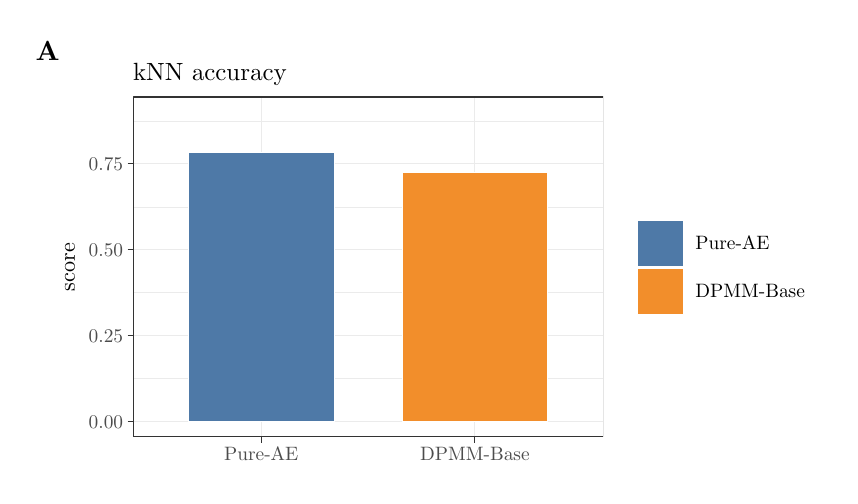
\begin{tikzpicture}[x=1pt,y=1pt]
\definecolor{fillColor}{RGB}{255,255,255}
\path[use as bounding box,fill=fillColor,fill opacity=0.00] (0,0) rectangle (289.70,161.83);
\begin{scope}
\path[clip] (  0.85,  1.74) rectangle (288.85,160.09);
\definecolor{drawColor}{RGB}{255,255,255}
\definecolor{fillColor}{RGB}{255,255,255}

\path[draw=drawColor,line width= 0.4pt,line join=round,line cap=round,fill=fillColor] (  0.85,  1.74) rectangle (288.85,160.09);
\end{scope}
\begin{scope}
\path[clip] ( 38.09, 13.93) rectangle (207.93,136.79);
\definecolor{fillColor}{RGB}{255,255,255}

\path[fill=fillColor] ( 38.09, 13.93) rectangle (207.93,136.79);
\definecolor{drawColor}{gray}{0.92}

\path[draw=drawColor,line width= 0.2pt,line join=round] ( 38.09, 35.03) --
	(207.93, 35.03);

\path[draw=drawColor,line width= 0.2pt,line join=round] ( 38.09, 66.05) --
	(207.93, 66.05);

\path[draw=drawColor,line width= 0.2pt,line join=round] ( 38.09, 97.08) --
	(207.93, 97.08);

\path[draw=drawColor,line width= 0.2pt,line join=round] ( 38.09,128.10) --
	(207.93,128.10);

\path[draw=drawColor,line width= 0.4pt,line join=round] ( 38.09, 19.52) --
	(207.93, 19.52);

\path[draw=drawColor,line width= 0.4pt,line join=round] ( 38.09, 50.54) --
	(207.93, 50.54);

\path[draw=drawColor,line width= 0.4pt,line join=round] ( 38.09, 81.57) --
	(207.93, 81.57);

\path[draw=drawColor,line width= 0.4pt,line join=round] ( 38.09,112.59) --
	(207.93,112.59);

\path[draw=drawColor,line width= 0.4pt,line join=round] ( 84.41, 13.93) --
	( 84.41,136.79);

\path[draw=drawColor,line width= 0.4pt,line join=round] (161.61, 13.93) --
	(161.61,136.79);
\definecolor{drawColor}{RGB}{255,255,255}
\definecolor{fillColor}{RGB}{78,121,167}

\path[draw=drawColor,line width= 0.3pt,fill=fillColor] ( 58.16, 19.52) rectangle (110.66,116.81);
\definecolor{fillColor}{RGB}{242,142,43}

\path[draw=drawColor,line width= 0.3pt,fill=fillColor] (135.36, 19.52) rectangle (187.86,109.49);
\definecolor{drawColor}{gray}{0.20}

\path[draw=drawColor,line width= 0.4pt,line join=round,line cap=round] ( 38.09, 13.93) rectangle (207.93,136.79);
\end{scope}
\begin{scope}
\path[clip] (  0.00,  0.00) rectangle (289.70,161.83);
\definecolor{drawColor}{gray}{0.30}

\node[text=drawColor,anchor=base east,inner sep=0pt, outer sep=0pt, scale=  0.70] at ( 34.49, 17.11) {0.00};

\node[text=drawColor,anchor=base east,inner sep=0pt, outer sep=0pt, scale=  0.70] at ( 34.49, 48.13) {0.25};

\node[text=drawColor,anchor=base east,inner sep=0pt, outer sep=0pt, scale=  0.70] at ( 34.49, 79.16) {0.50};

\node[text=drawColor,anchor=base east,inner sep=0pt, outer sep=0pt, scale=  0.70] at ( 34.49,110.18) {0.75};
\end{scope}
\begin{scope}
\path[clip] (  0.00,  0.00) rectangle (289.70,161.83);
\definecolor{drawColor}{gray}{0.20}

\path[draw=drawColor,line width= 0.4pt,line join=round] ( 36.09, 19.52) --
	( 38.09, 19.52);

\path[draw=drawColor,line width= 0.4pt,line join=round] ( 36.09, 50.54) --
	( 38.09, 50.54);

\path[draw=drawColor,line width= 0.4pt,line join=round] ( 36.09, 81.57) --
	( 38.09, 81.57);

\path[draw=drawColor,line width= 0.4pt,line join=round] ( 36.09,112.59) --
	( 38.09,112.59);
\end{scope}
\begin{scope}
\path[clip] (  0.00,  0.00) rectangle (289.70,161.83);
\definecolor{drawColor}{gray}{0.20}

\path[draw=drawColor,line width= 0.4pt,line join=round] ( 84.41, 11.93) --
	( 84.41, 13.93);

\path[draw=drawColor,line width= 0.4pt,line join=round] (161.61, 11.93) --
	(161.61, 13.93);
\end{scope}
\begin{scope}
\path[clip] (  0.00,  0.00) rectangle (289.70,161.83);
\definecolor{drawColor}{gray}{0.30}

\node[text=drawColor,anchor=base,inner sep=0pt, outer sep=0pt, scale=  0.70] at ( 84.41,  5.51) {Pure-AE};

\node[text=drawColor,anchor=base,inner sep=0pt, outer sep=0pt, scale=  0.70] at (161.61,  5.51) {DPMM-Base};
\end{scope}
\begin{scope}
\path[clip] (  0.00,  0.00) rectangle (289.70,161.83);
\definecolor{drawColor}{RGB}{0,0,0}

\node[text=drawColor,rotate= 90.00,anchor=base,inner sep=0pt, outer sep=0pt, scale=  0.80] at ( 17.05, 75.36) {score};
\end{scope}
\begin{scope}
\path[clip] (  0.00,  0.00) rectangle (289.70,161.83);
\definecolor{fillColor}{RGB}{255,255,255}

\path[fill=fillColor] (215.93, 54.02) rectangle (286.85, 96.71);
\end{scope}
\begin{scope}
\path[clip] (  0.00,  0.00) rectangle (289.70,161.83);
\definecolor{fillColor}{RGB}{255,255,255}

\path[fill=fillColor] (219.93, 75.36) rectangle (237.27, 92.71);
\definecolor{drawColor}{RGB}{255,255,255}
\definecolor{fillColor}{RGB}{78,121,167}

\path[draw=drawColor,line width= 0.3pt,fill=fillColor] (220.28, 75.72) rectangle (236.92, 92.35);
\end{scope}
\begin{scope}
\path[clip] (  0.00,  0.00) rectangle (289.70,161.83);
\definecolor{fillColor}{RGB}{255,255,255}

\path[fill=fillColor] (219.93, 58.02) rectangle (237.27, 75.36);
\definecolor{drawColor}{RGB}{255,255,255}
\definecolor{fillColor}{RGB}{242,142,43}

\path[draw=drawColor,line width= 0.3pt,fill=fillColor] (220.28, 58.37) rectangle (236.92, 75.01);
\end{scope}
\begin{scope}
\path[clip] (  0.00,  0.00) rectangle (289.70,161.83);
\definecolor{drawColor}{RGB}{0,0,0}

\node[text=drawColor,anchor=base west,inner sep=0pt, outer sep=0pt, scale=  0.70] at (241.27, 81.62) {Pure-AE};
\end{scope}
\begin{scope}
\path[clip] (  0.00,  0.00) rectangle (289.70,161.83);
\definecolor{drawColor}{RGB}{0,0,0}

\node[text=drawColor,anchor=base west,inner sep=0pt, outer sep=0pt, scale=  0.70] at (241.27, 64.28) {DPMM-Base};
\end{scope}
\begin{scope}
\path[clip] (  0.00,  0.00) rectangle (289.70,161.83);
\definecolor{drawColor}{RGB}{0,0,0}

\node[text=drawColor,anchor=base west,inner sep=0pt, outer sep=0pt, scale=  0.90] at ( 38.09,142.78) {kNN accuracy};
\end{scope}
\begin{scope}
\path[clip] (  0.00,  0.00) rectangle (289.70,161.83);
\definecolor{drawColor}{RGB}{0,0,0}

\node[text=drawColor,anchor=base,inner sep=0pt, outer sep=0pt, scale=  1.00] at (  7.20,150.08) {\bfseries A};
\end{scope}
\end{tikzpicture}
